\documentclass[border=10pt]{standalone}
\usepackage[siunitx]{circuitikz}
\begin{document}
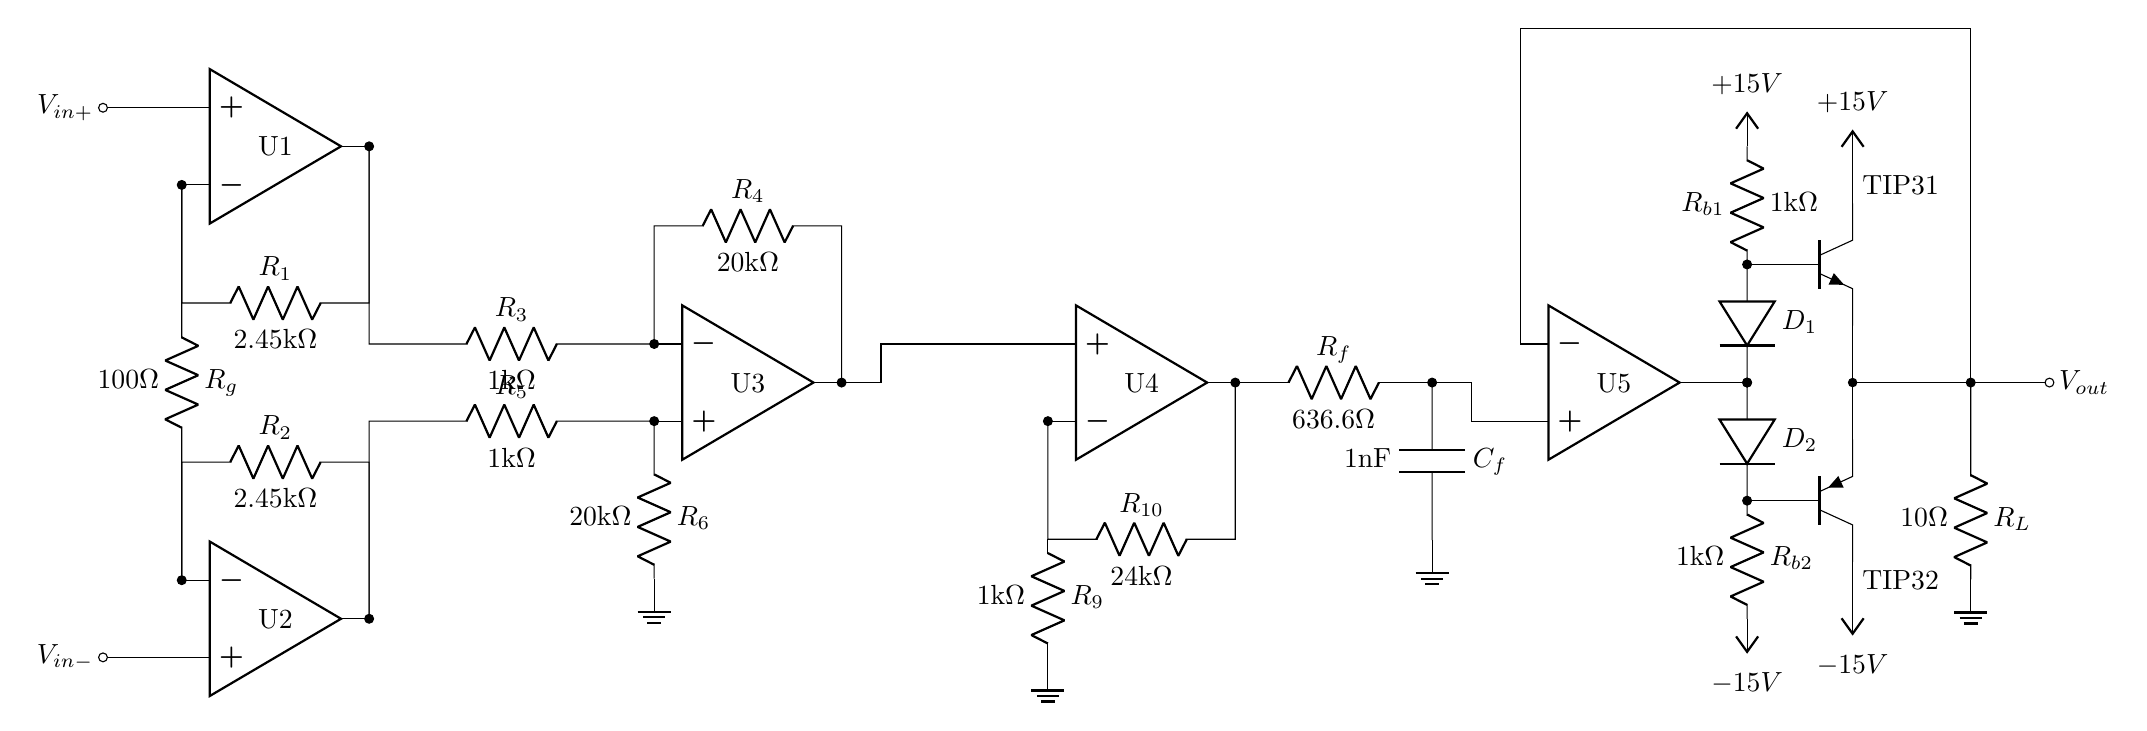
\begin{tikzpicture}[scale=1, transform shape]

% --- ETAPA 1: Entrada Diferencial ---

% U1 (Top, V_in+)
\draw (0, 3) node[op amp, yscale=-1] (u1) {}; 
\node at (u1.center) {U1};
\draw (u1.+) to[short, -o] ++(-1,0) node[left] {$V_{in+}$};

% U2 (Bottom, V_in-)
\draw (0, -3) node[op amp] (u2) {}; 
\node at (u2.center) {U2};
\draw (u2.+) to[short, -o] ++(-1,0) node[left] {$V_{in-}$};

% Rg
\draw (u1.-) to[R, l=$R_g$, a=100\(\Omega\)] (u2.-);

% Feedback U1
\draw (u1.-) to[short, *-] ++(0, -1.5) coordinate (fb1_bot)
      to[R, l=$R_1$, a=2.45k\(\Omega\)] (fb1_bot -| u1.out)
      to[short, -*] (u1.out);

% Feedback U2
\draw (u2.-) to[short, *-] ++(0, 1.5) coordinate (fb2_top)
      to[R, l=$R_2$, a=2.45k\(\Omega\)] (fb2_top -| u2.out)
      to[short, -*] (u2.out);


% --- ETAPA 2: Amplificador Diferencial ---

\draw (6, 0) node[op amp] (u3) {};
\node at (u3.center) {U3};

% Resistencias de entrada a U3
\draw (u1.out) -- (u1.out |- u3.-) to[R, l=$R_3$, a=1k\(\Omega\)] (u3.-);
\draw (u2.out) -- (u2.out |- u3.+) to[R, l=$R_5$, a=1k\(\Omega\)] (u3.+);

% Feedback U3
\draw (u3.-) to[short, *-] ++(0, 1.5) coordinate (fb3_top)
      to[R, l=$R_4$, a=20k\(\Omega\)] (fb3_top -| u3.out)
      to[short, -*] (u3.out);

% Grounding U3.+
\draw (u3.+) to[short, *-] ++(0, -0.5) 
      to[R, l=$R_6$, a=20k\(\Omega\)] ++(0, -1.5) node[ground]{};


% --- ETAPA 3: Etapa de Ganancia (No Inversor) ---

\draw (11, 0) node[op amp, yscale=-1] (u4) {}; 
\node at (u4.center) {U4};

% Conexion de U3 a U4
\draw (u3.out) -- ++(0.5, 0) |- (u4.+);

% Feedback U4
\draw (u4.-) to[short, *-] ++(0, -1.5) coordinate (fb4_bot)
      to[R, l=$R_{10}$, a=24k\(\Omega\)] (fb4_bot -| u4.out) to[short, -*] (u4.out);
\draw (fb4_bot) to[R, l=$R_9$, a=1k\(\Omega\)] ++(0, -1.5) node[ground]{};


% --- ETAPA 4: Filtro Pasa Bajos RC ---

\draw (u4.out) to[R, l=$R_f$, a=636.6\(\Omega\)] ++(2.5, 0) coordinate (filt_node);
\draw (filt_node) to[C, l=$C_f$, a=1nF, *-] ++(0, -2) node[ground]{};


% --- ETAPA 5: Buffer y Push-Pull ---

\draw (17, 0) node[op amp] (u5) {};
\node at (u5.center) {U5};

% Conexion del filtro al buffer
\draw (filt_node) -- ++(0.5, 0) |- (u5.+);

% Red de Diodos
\draw (u5.out) to[short] ++(0.5, 0) coordinate (op5_out);
\path (op5_out) ++(0, 1.5) coordinate (base_npn);
\path (op5_out) ++(0, -1.5) coordinate (base_pnp);

\draw (base_npn) to[D, l=$D_1$, *-*] (op5_out);
\draw (op5_out) to[D, l=$D_2$, *-*] (base_pnp);

% Biasing
\draw (base_npn) to[R, l=$R_{b1}$, a=1k\(\Omega\)] ++(0, 1.5) node[vcc]{$+15V$};
\draw (base_pnp) to[R, l=$R_{b2}$, a=1k\(\Omega\)] ++(0, -1.5) node[vee]{$-15V$};

% Transistores de Salida
\draw (base_npn) -- ++(0.5, 0) node[npn, anchor=B] (q1) {};
\draw (base_pnp) -- ++(0.5, 0) node[pnp, anchor=B] (q2) {};
\node[above right] at (q1.C) {TIP31};
\node[below right] at (q2.C) {TIP32};

\draw (q1.C) -- ++(0, 0.5) node[vcc]{$+15V$};
\draw (q2.C) -- ++(0, -0.5) node[vee]{$-15V$};

% Union de emisores
\draw (q1.E) -- (q2.E) coordinate[midway] (out_final);
\filldraw (out_final) circle (1.5pt);

% Nodo de salida y carga
\draw (out_final) -- ++(1.5, 0) coordinate (out_node);
\draw (out_node) to[short, -o] ++(1, 0) node[right]{$V_{out}$};
\draw (out_node) to[short, *-] ++(0, -1) to[R, l=$R_L$, a=10\(\Omega\)] ++(0, -1.5) node[ground]{};

% Realimentacion Global de U5
\draw (out_node) -- ++(0, 4.5) coordinate (fb5_top) 
      -- (fb5_top -| u5.-) -- (u5.-);

\end{tikzpicture}
\end{document}
